\section{Komplexe Funktion, Abbildungen}
	\begin{minipage}[t]{0.5\textwidth}
		\subsection{Definition}
			%\scalebox{0.65}{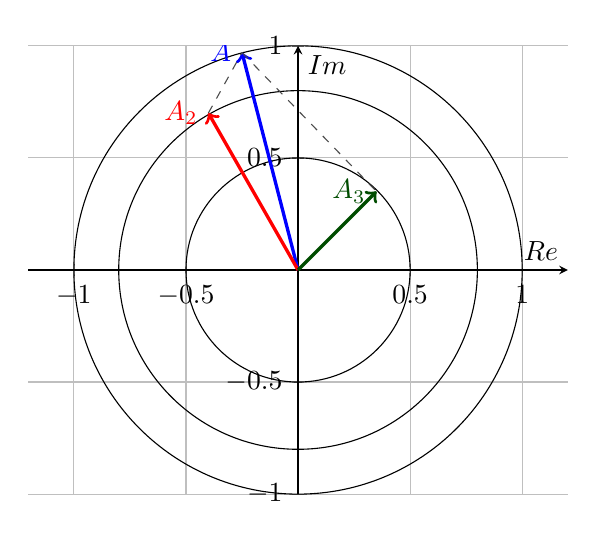
\begin{tikzpicture}
	%\draw[help lines] (0,0) grid (6,4);
	\begin{axis}[axis lines=middle, axis equal, grid=both, xmin=-1, xmax=1, ymin=-1, ymax=1, xlabel = $\operatorname{Re}$, ylabel = $\operatorname{Im}$]
		\draw (axis cs: 0, 0) circle [blue, radius=1];
		\draw (axis cs: 0, 0) circle [red, radius=0.8];
		\draw (axis cs: 0, 0) circle [black!70!green, radius=0.5];
		\addplot[->, blue, very thick] coordinates{(0, 0) (-0.25, 0.97)}  node[sloped, above, blue, left] {$A$};
		\addplot[->, red, very thick] coordinates{(0, 0) (-0.4, 0.7)}  node[sloped, above, red, left] {$A_2$};
		\addplot[->, black!70!green, very thick] coordinates{(0, 0) (0.35, 0.35)}  node[sloped, above, black!70!green, left] {$A_3$};
		\addplot[dashed, black!70] coordinates{(-0.4, 0.7) (-0.25, 0.97)};
		\addplot[dashed, black!70] coordinates{(-0.25, 0.97) (0.35, 0.35)};
	\end{axis}
\end{tikzpicture}}
	\end{minipage}
	\begin{minipage}[t]{0.5\textwidth}
		\subsection{Winkeltreue}
			Komplexe Funktion $\operatorname{f}\left( z \right)$ ist in allen Punkten winkeltreu, wo gibt: \fbox{$\operatorname{f}^{\prime}\left( z \right) \neq 0$}\\[6pt]
			Sie bewirkt \textbf{lokal eine Drehstreckung:}\\[3pt]
			\begin{tabular}{ll}
				Streckungsfaktor: & \fbox{$\left|f^{\prime}(z)\right|$}\\[3pt]
				Drehwinkel: & \fbox{$\operatorname{\arg}\left( z \right)$}\\[3pt]
			\end{tabular}
	\end{minipage}
\subsection{Parameter- und Koordinatengleichung}
	\begin{minipage}[t]{0.2\textwidth}
		
	\end{minipage}
	\begin{minipage}[t]{0.8\textwidth}
		\begin{tabular}{llll}
			\textbf{waagrechte Gitternetzlinien durch Punkt $(0; c_2)$:} & &\\[3pt]
		\end{tabular}
		\begin{tabular}{llll}
			\fbox{$z = \operatorname{z}\left( r \right) = r + \mathrm{j} c_2$} & $\xrightarrow[]{\operatorname{f}\left( z \right)}$ & \fbox{$w = \operatorname{w}\left( r \right) = \operatorname{f}\left( \operatorname{z}\left( r \right) \right) = \operatorname{f}\left( r + \mathrm{j} c_2 \right)$} & mit $r \subset \mathbb{R}$\\[3pt]
		\end{tabular}
		\begin{tabular}{llll}
			\textbf{senkrechte Gitternetzlinien durch Punkt $(c_1; 0)$:} & & &\\[3pt]
		\end{tabular}
		\begin{tabular}{llll}
			\fbox{$z = \operatorname{z}\left( r \right) = c_1 + \mathrm{j} r$} & $\xrightarrow[]{\operatorname{f}\left( z \right)}$ & \fbox{$w = \operatorname{w}\left( r \right) = \operatorname{f}\left( \operatorname{z}\left( r \right) \right) = \operatorname{f}\left( c_1 + \mathrm{j} r \right)$} & mit $r \subset \mathbb{R}$\\[3pt]
		\end{tabular}
		\begin{tabular}{llll}
			\textbf{Koordinatengleichung:} & 
			\fbox{$\left| \begin{array}{c}
				w_1 = \operatorname{Re}\left(\left[ \operatorname{f}\left(\operatorname{z}\left(r \right)\right)\right]\right)\\[3pt]
				w_2 = \operatorname{Re}\left(\left[ \operatorname{f}\left(\operatorname{z}\left(r \right)\right)\right]\right)
				\end{array} \right|$} &
			$\Rightarrow$ & 
			$\begin{array}{l}
				\text{Parameter $r$ eliminieren,}\\[3pt]
				\text{um Koordinatengleichung}\\[3pt]
				\text{zu erhalten.}
			\end{array}$
		\end{tabular}
	\end{minipage}

\subsection{Lineare Funktion}
	\begin{minipage}[t]{0.5\textwidth}
		
	\end{minipage}
	\begin{minipage}[t]{0.5\textwidth}
		Die lineare Funktion $w = \operatorname{f}\left( z \right) = a z + b$ bewirkt:\\[3pt]
		\renewcommand{\arraystretch}{1.7}
		\begin{tabular}{|lll|}
			\hline
			Drehstreckung mit: & Streckungsfaktor & $\left|a\right|$\\
	 & Drehwinkel & $\operatorname{arg}\left( a \right)$\\
	 & Zentrum & $\dfrac{b}{1-a}$\\[6pt]
			\hline
			Drehstreckung mit: & Streckungsfaktor & $\left|a\right|$\\
			& Drehwinkel & $\operatorname{arg}\left( a \right)$\\
			\textbf{und} Translation um: & Ortsvektor & $b$\\
			\hline
		\end{tabular}
	\renewcommand{\arraystretch}{1}
	\end{minipage}\\[3pt]
	\begin{minipage}[t]{0.7\textwidth}
		\textbf{Parametergleichung:}\\[3pt]
		\begin{tabular}{lcl}
			Waagrechte & $\xrightarrow[]{\operatorname{f}\left( z \right)}$ & $w = w(r) = \underbrace{\left( \mathrm{j} a c_2 + b \right)}_{Startvektor} + \hspace{25pt} r \cdot \hspace{-28pt} \underbrace{a}_{Richtungsvektor}$\\[3pt]
			Senkrechte & $\xrightarrow[]{\operatorname{f}\left( z \right)}$ & $w = w(r) = \underbrace{\left( a c_1 + b \right)}_{Startvektor} + \hspace{25pt} r \cdot \hspace{-25pt} \underbrace{\mathrm{j}a}_{Richtungsvektor}$\\[3pt]
		\end{tabular}
	\end{minipage}
	\begin{minipage}[t]{0.3\textwidth}
		\textbf{Parametergleichung:}\\[3pt]
		$\operatorname{f}^{\prime}\left( z \right) = a$\\[3pt]
		\begin{tabular}{ll}
			$\Rightarrow$ & für $a \neq 0$ ist $\operatorname{f}\left( z \right) = a z + b$\\[3pt]
	 & \textbf{überall winkeltreu!}
		\end{tabular}
	\end{minipage}

\section{Potenzfunktion und Wurzelfunktion}
	\subsection{Quadratfunktion $z^2$ und Wurzelfunktion $\sqrt{z}$}
		Beim Quadrieren wird das \textbf{Argument verdoppelt} $\Rightarrow$ halbe $z$-Ebene füllt bereits die ganze $w$-Ebene aus.\\[3pt]
		
		\begin{minipage}[t]{0.5\textwidth}
			\begin{framed}
				Die Quadratfunktion $w = \operatorname{f}\left( z \right) = z^2$ bildet die\\[3pt]
				$z$-Ebene bijektiv \textbf{auf eine zweiblättrige\\[3pt] Riemann'sche Fläche ab}.
			\end{framed}
		\end{minipage}
		\begin{minipage}[t]{0.5\textwidth}
			
		\end{minipage}\\[3pt]
		\begin{minipage}[t]{0.2\textwidth}
			\textbf{Winkeltreue:}
		\end{minipage}
		\begin{minipage}[t]{0.5\textwidth}
			\begin{framed}
				\begin{tabular}{lll}
					$\operatorname{f}^{\prime}\left( z \right) = 2 z$ & $\Rightarrow$ & \textbf{winkeltreu} ausser bei $z = 0$\\[3pt]
					$\operatorname{f}^{-1}\left( w \right) = \sqrt{w}$ & $\Rightarrow$ & \textbf{winkeltreu} ausser bei $w = 0$\\[3pt]
				\end{tabular}
			\end{framed}
		\end{minipage}
		\begin{minipage}[t]{0.3\textwidth}
			
		\end{minipage}\\[3pt]
	
	\subsection{Potenzfunktion $z^n$ und Wurzelfunktion $\sqrt[n]{z}$}
		\begin{minipage}[t]{0.5\textwidth}
			\begin{framed}
				Die Potenzfunktion $w = \operatorname{f}\left( z \right) = z^n$ bildet die\\[3pt]
				$z$-Ebene bijektiv \textbf{auf eine n-blättrige\\[3pt] Riemann'sche Fläche ab}.
			\end{framed}
		\end{minipage}
		\begin{minipage}[t]{0.5\textwidth}
			
		\end{minipage}\\[3pt]
\section{Kreisspiegelung}
	\begin{minipage}[t]{0.5\textwidth}
		\begin{tabular}{lll}
			\fbox{$w = \overline{\operatorname{f}}\left( z \right) = \dfrac{1}{\overline{z}}$} &
			mit: $|w| = \dfrac{1}{\left| z \right|}$; &
			$\operatorname{arg}\left( w \right) = \operatorname{arg}\left( z \right)$\\[3pt]
		\end{tabular}
	\end{minipage}
	\begin{minipage}[t]{0.5\textwidth}
		
	\end{minipage}\\[3pt]
	\begin{minipage}[t]{0.05\textwidth}
		\vspace{17pt}
		$\Rightarrow$ 
	\end{minipage}
	\begin{minipage}[t]{0.55\textwidth}
		\textbf{Kreisspiegelung bedeutet: symmetrisch}\\[3pt]
		\textbf{bezüglich des Einheitskreises (Reziprokwert)}\\[3pt]
		Das Innere des Einheitskreises wird auf das Äussere\\[3pt]
		abgebildet und umgekehrt.
	\end{minipage}
	\begin{minipage}[t]{0.4\textwidth}
		
	\end{minipage}\\[3pt]

\subsection{Regeln bei der Kreisspiegelung}
	\fbox{
		\begin{tabular}{ll}
			\textbf{Winkeltreue:} & Die Kreisspiegelung ist \textbf{überall winkeltreu!}
		\end{tabular}
	}\\[3pt]
	\fbox{
		\begin{tabular}{ll}
			\textbf{Kreistreue:} & Die Kreisspiegelung ist kreistreu (Geraden sind Kreise mit $r = \infty$)
		\end{tabular}
	}\\[3pt]
	\begin{tabular}{|c|c|c|c|c|}
		\hline
		\textbf{Originalkurve:} & \textbf{Bildkurve:} & & \textbf{Originalkurve:} & \textbf{Bildkurve:}\\
		\hline
		%\includegraphics{} & \includegraphics{} & & \includegraphics{} & \includegraphics{}\\
		\hline
		%\includegraphics{} & \includegraphics{} & & \includegraphics{} & \includegraphics{}\\
		\hline
	\end{tabular}\\[3pt]
	\begin{minipage}[t]{0.5\textwidth}
		\subsection{Konstruktion von Bildpunkten}
			\begin{minipage}[t]{0.5\textwidth}
				$z$ \textbf{innerhalb des Einheitskreises}:\\[3pt]
				
			\end{minipage}
			\begin{minipage}[t]{0.5\textwidth}
				$z$ \textbf{ausserhalb des Einheitskreises}:\\[3pt]
				
			\end{minipage}
	\end{minipage}
	\begin{minipage}[t]{0.5\textwidth}
		\subsection{Exponentialfunktion $\mathrm{e}^z$}
			\begin{minipage}[t]{0.3\textwidth}
				\fbox{$\mathrm{e} = \mathrm{e}^z_1 + \operatorname{cjs}\left( z_2 \right)$}
			\end{minipage}
			\begin{minipage}[t]{0.7\textwidth}
				\begin{tabular}{lcl}
					\textbf{Waagrechte} & $\rightarrow$ & \textbf{Strahlen}\\[3pt]
					\textbf{Senktrechte} & $\rightarrow$ & \textbf{Kreise um $\mathrm{O}$}\\[3pt]
				\end{tabular}
		\end{minipage}
		\end{minipage}